\section{Tail mathematical model}
In order to devise a mathematical model of tail dynamics, we propose modeling the tail as a kinematic chain manipulator attached to robot body. Much like in aerial robots, when the robot is in the air, the tail acts frealy on its body. We propose using the tail as a dynamic stabilizator for the hopping. First we build the kinematic model using Denavit-Hartenberg parametrization metod, after that we devise a dynamic model of the arms using recursive Newton-Euler algorithm.

\subsection{Kinematic model}
Kinematic chain of the tail is shown in Fig. \ref{fig:rmax}, and the kinematic parameters are shown in table \ref{tab:DHParameters}. Kinematic chain consists of the body coordinate system, 2 revolute joints on of the tail, one virtual prismatic joint in the tail (i.e. Tail length parameter), and the tail tip coordinate system. As can be seen from DH parameters table, the two revolute joints have no linear, only angular dislacement from each other, therefore their masses and moments of inertia are all zero. The third prismatic joint represents the tail length and is modeled as a long stick with infitesimal thickness. Its moment of inertia is, therefore, written as:

\begin{equation}
J_3=\frac{{Q_3}^2 m_3}{12}\left(
\begin{array}{ccc}
 1 & 0 & 0 \\
 0 & 1 & 0 \\
 0 & 0 & 0
\end{array}
\right)
\end{equation} 

\begin{table}
	\centering
		\begin{tabular}{ccccc}
		\hline
			& $\theta$ & $d$ & $a$ & $\alpha$ \\\hline
			\multicolumn{5}{c}{Body}\\\hline
			$B-0$ & $0$ & $d_B$ & $a_B$ & $0$\\\hline
			\multicolumn{5}{c}{Tail}\\\hline
			Joint 1 & $q_1$ & $0$ & $0$ & $-\frac{\pi}{2}$\\
			Joint 2 & $q_2$ & $0$ & $0$ & $\frac{\pi}{2}$\\
			Virtual joint& $0$ & $q_3$ & $0$ & $0$\\\hline
		\end{tabular}
	\caption{Denavit-Hartenberg Parameters}\label{tab:DHParameters}
\end{table}

\begin{multicols}{2}
\begin{equation}
\tau_b=\begin{bmatrix}
\frac{1}{24} m_3 Q_3 \left(-12 g S_1 S_2+Q_3 \left(3 S_1 S2_2 {\dot{Q}_1}^2-2 C_1\left(5+3 C2_2\right) \dot{Q}_1 \dot{Q}_2-3 C_1 S2_2 \ddot{Q}_1-8 S_1 \ddot{Q}_2\right)\right)\\
\frac{1}{24} m_3 Q_3 \left(-12 g C_1 S_2+Q_3 \left(S_1\left( 2(5+3C2_2)\dot{Q}_1 \dot{Q}_2+3S2_2\ddot{Q}_1\right)+C_1(3S2_2{\dot{Q}_1}^2-8\ddot{Q}_2)\right)\right)\\
\frac{1}{4} S_2 m_3 Q_3^2 \left(2 C_2 \dot{Q}_1 \dot{Q}_2+S_2 \ddot{Q}_1\right)
\end{bmatrix}
\end{equation}
\end{multicols}

\begin{figure}
	\centering
	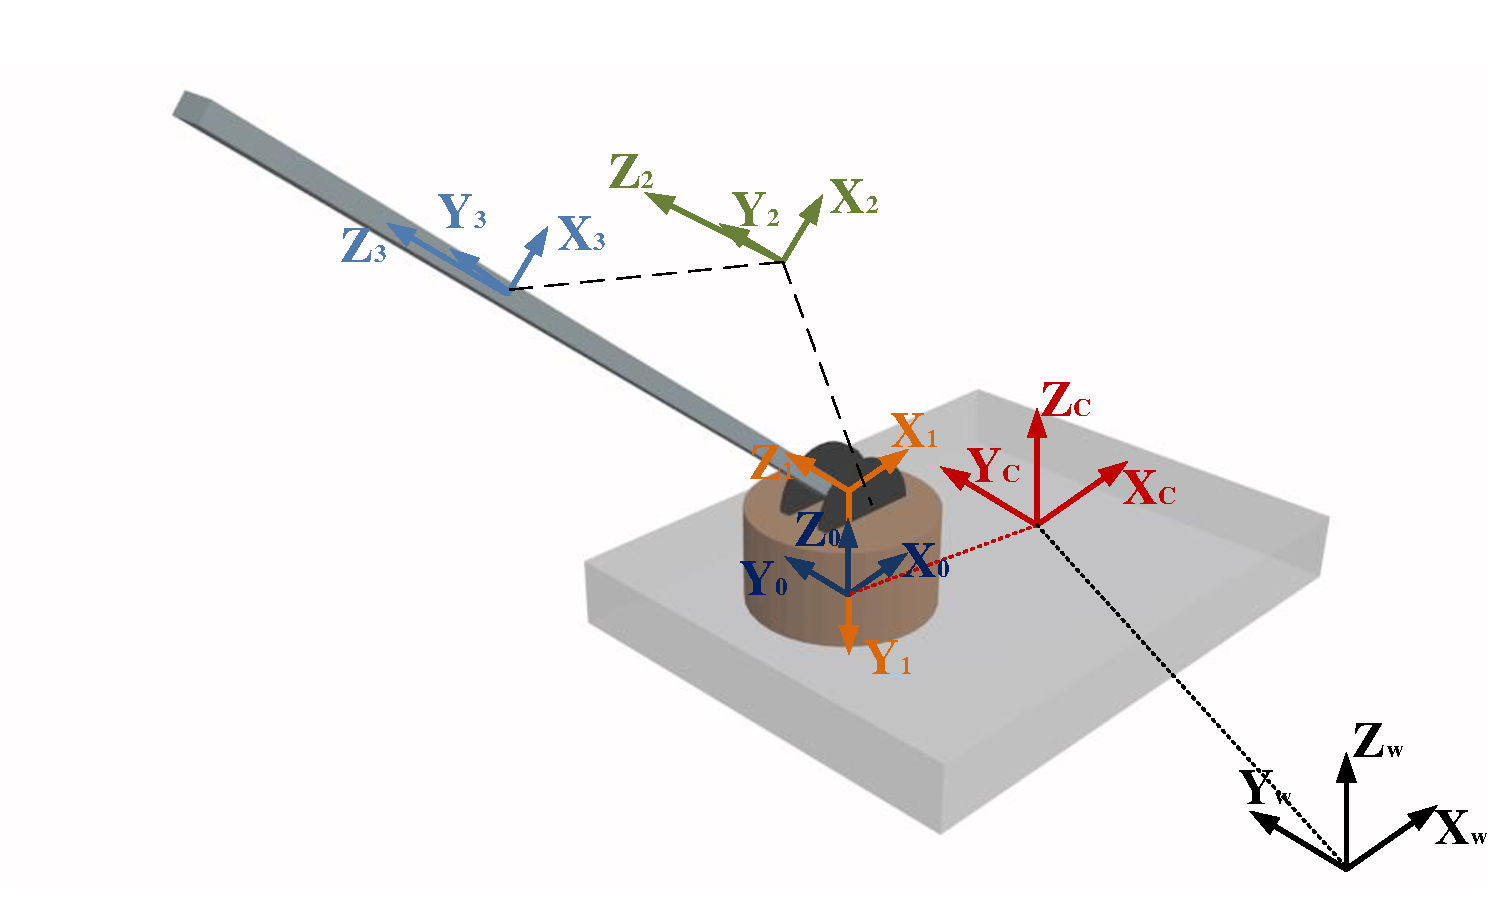
\includegraphics[width=85mm]{./pictures/RobinRepic.pdf}
	\caption{Robin Tail kinematic chain model}
	\label{fig:rmax}
\end{figure}

\begin{figure}
	\centering
	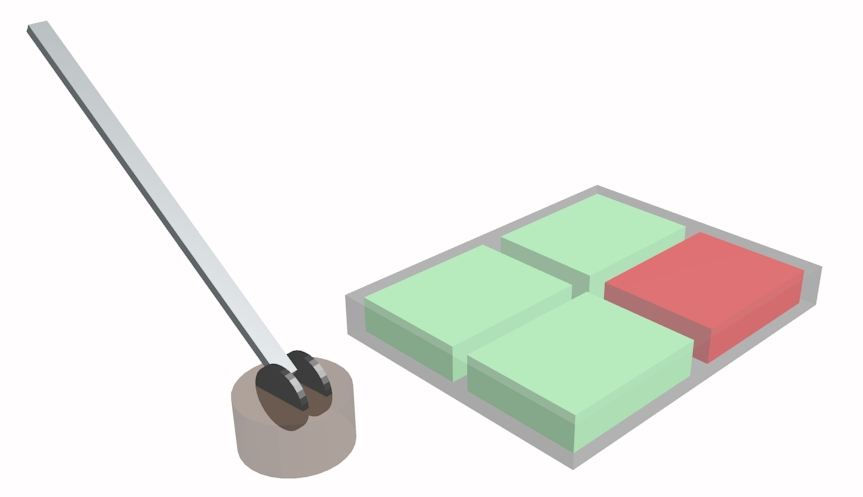
\includegraphics[width=85mm]{./pictures/RobinMoment.jpg}
	\caption{Robin moment}
	\label{fig:rmoment}
\end{figure}
